From our point of view, there are several requirements that the model
should be able to fulfill. Namely:

\begin{itemize}
  \item good support for deformations by bending and twisting
  \item the results of the deformation should be global
  \item method should allow arbitrary models and not rely on specific
  structure of the object (e.g. on tubular structure like \cite{Li2009})
  \item the model has to be able to deal with collisions (e.g. between the
  aortic arch and pulmonary artery)
\end{itemize}

Several different models are commonly used for modelling thin structures or
tubular-like structures resembling blood vessels. \tomas{Add refs. or
reformulate!} For the predictive simulation of the surgery we choose to use
thin shell elements, because in our opinion it satisfies all the
requirements very well. They are very often considered numerically too
expensive, this is however not necessarily true.

\tomas{image: single shell}

The formulation of the thin shell elements is based on the mechanics of
continuum. These elements are commonly used in physics and mechanics for
deformation modelling of thin structures because they are numerically more
stable then volumetric FEM methods in this situation. The shell element is
a 2-dimensional element whose thickness is a parameter of the simulation.
Often the thickness is considered constant over the surface of the element.
Shell combines forces from in-plane deformations, like stretching or
shearing, with bending forces. Such internal forces $\myvec{f}$ are a
function of current displacement measured as difference of current shape
$\myvec{x}$ from the rest shape $\myvec{x_0}$.

\begin{equation}
  \myvec{f} = K(\myvec{x} - \myvec{x_0})
\end{equation}

For more thorough description we refer the reader to the textbook about
Finite Elements for example \tomas{add ref}.

In the rest of the section we want to show that the performance of a model
based on the shell element is adequate for the simulation.

\begin{figure}[tbh]
  \begin{minipage}[b]{0.3\linewidth}
      \framebox[1cm]{\rule{0pt}{1cm}}
      %\includegraphics[width=\columnwidth]{img/}
      \caption{Bending shell element}
      \label{fig-shell}
  \end{minipage}
  \hspace{0.1\columnwidth}
  \begin{minipage}[b]{0.6\linewidth}
    \centering
    \begin{tabular}{cc}
     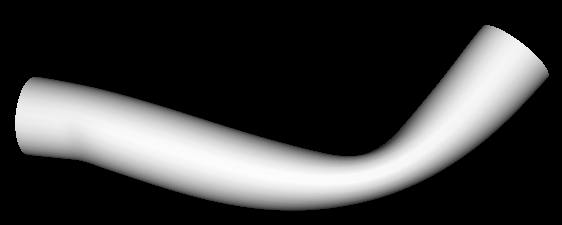
\includegraphics[width=0.5\columnwidth]{img/compare-bend.png}
      &
      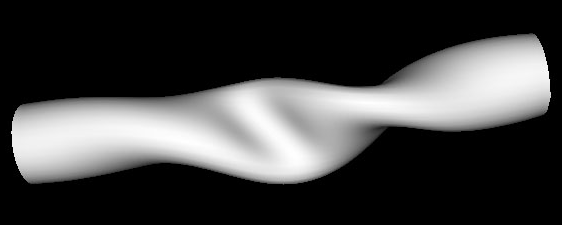
\includegraphics[width=0.5\columnwidth]{img/compare-twist.png}
      \\
      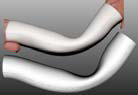
\includegraphics[width=0.5\columnwidth]{img/compare-bend-other.png}
      &
      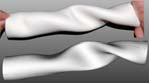
\includegraphics[width=0.5\columnwidth]{img/compare-twist-other.png}
    \end{tabular}
    \caption{Bending and twisting deformations. Upper: shell model; middle:
    artificial tube, bottom: Cosserat rod \cite{Li2009}. (Credits for the
    bottom images: Li et al.)}
    \label{fig-deformations}
  \end{minipage}
\end{figure}

Figure \ref{fig-deformations} shows different deformations that are likely to
occur during the surgery (bending and twisting). The figure compares our
results with the results of Li et al. \cite{Li2009}. As you can see the
results are closer to the real deformations.

The bending property of the shell allows us to use smaller number of
elements for the simulation and use high polygonal model only for
visualisation. The convergence of the model is a key factor here. In our experiments we
were able to use only as few as eight nodes around the circumference of a
tubular model while still maintaining realistic behaviour. Figure
\tomas{add-ref} shows the results for different number of nodes along the
circumference.

\tomas{image: convergence}

We have used the model of Olivier Comas \cite{Comas2010b,Comas2010c} and
also our own model. But our method described in section \ref{sec-method}
does not depend on any particular model. Since we use the method as a
geometrical tool we have also certain independence on physical parameters.
For example the variation of Young's modulus in the interval from $10^3$ to
$10^7$ resulted to only $0.1\%$ change of the deformation.


% vim: et sw=2 tw=75 fdm=marker fdc=2 spell
